\section{Geo-Datenbanken}
\label{sec:Datenbanken}

Die Speicherung, Verwaltung und Verarbeitung von Daten haben für viele Anwendungsbereiche eine große Bedeutung.  Wie \cite{brinkhoff_geodatenbanksysteme_2022} in seinem Werk über Geodatenbanksysteme erwähnt, erfüllen diese speziellen Datenbanken eine Vielzahl an Aufgaben. Sie müssen nicht nur allgemeine Anforderungen wie Sicherheit, Mehrbenutzerfähigkeit und Effizienz erfüllen, sondern auch spezifische geoinformationssystemische Funktionen bieten. Dazu gehören die Verwaltung von Geometriedaten und deren Verarbeitung. Zudem stellen sie Werkzeuge für die räumlichen Analyse von Geoobjekten bereit und halten sich an Standards, um eine möglichst große Interoperabiltät zu gewährleisten. \\

\textbf{Definition: }Eine Geodatenbank ist eine Datenbank, welche für die Verarbeitung von räumlichen Daten optimiert ist. [...] Geodatenbanken entstehen oft durch die Erweiterung klassischer Datenbanksysteme mit entsprechender Software. Bekannte Ausführungen sind MongoDB with GeoJSON, PostgreSQL with PostGIS, SpatiaLite with Sqlite, Oracle Spatial and Graph etc. \citep{wiki-geodatenbank}.\\

In der Abbildungen 2.2 und 2.3 (eigene Darstellung) wird ein Unterschied der Speicherung von Geodaten gezeigt. Die beide Abbildungen zeigen Tabellen aus einer Geodatenbank, wobei der Hauptunterschied in der Art und Weise liegt, wie die geographischen Koordinaten gespeichert sind. In der ersten Bild werden Koordinaten als separate Spalten für den Längengrad und den Breitengrad aufgeführt. Jede Zeile enthält nummerische Werte für diese Koordinaten, die die genaue Position auf der Erde repräsentiert. Im zweiten Bild wird stattdessen eine Spalte koordinaten mit einem speziellen Geometriedatentyp hinterlegt. Hier sind die Koordinaten als 'POINT' gespeichert. Für jeden Eintrag wird ein Punkt mit dem jeweiligen Längen- und Breitengraden in Klammern angegeben 'POINT(13.357818 52.49637)'. \\

\begin{figure}[ht]
  \centering
  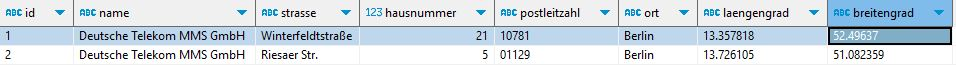
\includegraphics[width=\linewidth]{images/einfacheDB.jpg}
  \caption{Geodaten in der Datenbank. How (not) to}
  \label{fig:meineabbildung}
\end{figure}
\begin{figure}[ht]
  \centering
  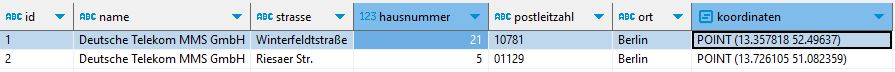
\includegraphics[width=\linewidth]{images/geoDB.jpg}
  \caption{Geodaten in der Datenbank mit Geo-Erweiterug. How to}
  \label{fig:meineabbildung}
\end{figure}
 Die Geodatenbank haben drei Aspekte, die räumliche Daten mit einer Datenbank zu verknüpfen: Datentypen, Indizes und Funktionen.
\begin{enumerate}
    \item Räumliche Datentypen beziehen sich auf spezialisierte Datenformate, die zur Speicherung von Geodaten verwendet werden. Dies Datentypen repräsentieren unterschiedliche geographische Elemente und Formen - Punkt (POINT), Linie (LineString) und Polygon (POLYGON).
    \item Die mehrdimensionale räumliche Indizierung ist eine Funktion, die es ermöglicht, räumliche Daten effizient zu organisieren und zu durchsuchen. Diese Indizes sind speziell für die Verarbeitung von Geodaten konzipiert und optimieren Abfragen, die sich auf die Positionen, den Abstand oder Überlappung von Geoobjekten beziehen. Sie beschleunigen die Suchanfragen, indem sie nur die relevanten Teile der Datenbank durchsuchen, anstatt jeden Datensatz einzeln zu prüfen.
    \item Räumliche Funktionen umfassen eine Sammlung von Operationen und Abfragen, die in SQL bereitgestellt sind. Dies Funktionen können verwendet werden, um räumliche Beziehungen zu bestimmen, wie z.B. zu prüfen, ob ein Punkt in einem Polygon liegt, Lienen sich kreuzen oder die nächstgelegenen Objekte zu einem gegebenen Punkt zu finden. Sie ermöglichen es, komplexe räumliche Fragen direkt in der Datenbank zu beantworten. 
\end{enumerate}

Geodatenbanken ermöglichen durch die klassischen SQL-Befehlen Beziehungen zwischen Geometrie zu analysieren bzw. neue Geometrien zu erstellen wie beispielsweise Berechnungen von Längen, Distanzen, Prüfungen auf Bedingungen wie maximaler Abstand, Erstellung neuer Geometrien etc.
